\documentclass[11pt]{article}
\usepackage[T1]{fontenc}
\usepackage[margin=1in]{geometry}
\usepackage{amsmath,amssymb,amsthm}
\usepackage{graphicx}
\usepackage[colorlinks=true,linkcolor=blue,citecolor=blue,urlcolor=blue]{hyperref}
\newtheorem{definition}{Definition}[section]
\newtheorem{conjecture}[definition]{Conjecture}
\theoremstyle{remark}
\newtheorem{remark}[definition]{Remark}
\newcommand{\Tr}{\operatorname{Tr}}
\newcommand{\Erec}{E^{\rm Petz}_{\rm rec}}

\title{Recoverability Length Scales and Wilson Loops in Lattice Gauge
Theories\\
{\large Protocol, definitions, and conjectural links to confinement
diagnostics}\\
{\normalsize Version 2}}
\author{Lluis Eriksson\\ Independent Researcher\\ \texttt{lluiseriksson@gmail.com}}
\date{January 2026 (v1); July 2026 (v2)}

\begin{document}
\maketitle

\begin{abstract}
We propose a numerical protocol and falsifiable conjectures relating
quantum-information recoverability measures to confinement diagnostics in
lattice gauge theories. For a tripartition $A$--$B$--$C$ and collar width
$w$, we define a Petz-type recovery error $\Erec(w)$ and extract a
recoverability length from threshold and fit criteria. Since gauge
constraints obstruct naive factorization, the protocol is formulated in an
extended-Hilbert-space (EHS) prescription by default, with an algebraic
(gauge-invariant) variant outlined together with its subtleties (centers,
sectors). We conjecture that $\Erec(w)$ decays exponentially in gapped
phases and that its scale tracks confinement scales set by Wilson loops.
\emph{v2 executes the testbed that v1 only specified:} on a $\mathbb{Z}_2$
ladder of four plaquettes (13 links, Gauss law enforced exactly,
$\langle G_v \rangle = 1$ to $10^{-6}$), the suite computes $\Erec(w)$ and
Wilson decay on the same ground states across five couplings. Findings:
the pipeline runs end to end; $\xi_{\rm rec}$ is identifiable at three of
five couplings and nearly coupling-independent ($0.20$--$0.27$, spread
$\times 1.3$), while the Wilson decay length varies strongly ($1.2$--$6.9$,
spread $\times 5.8$ over the fittable set): \emph{no tracking at ladder level}. Because
height-one ladders degenerate area and perimeter, the Wilson scale there
is not a pure confinement scale, so this first dataset is
inconclusive-but-cautionary for the tracking conjecture rather than a
falsification -- and it sharpens the requirement: a genuine 2D lattice is
needed. v2 further flags the TFIM control row shared with the companion
framework note as unstable under regeneration, and adds series
positioning. No v1 definition is changed.
\end{abstract}

\section{Introduction, preliminaries, prescriptions, definitions}
As in v1 (unchanged): squared Uhlmann fidelity and $E_{\rm rec} = -\log
F$; EHS prescription as default (reduced states are ordinary density
matrices; edge modes on cut links) with the algebraic prescription
outlined (centers, sector-wise fidelity/recovery) \cite{Donnelly, CHR};
regularized Petz-type map (CP, trace-normalized output; used as an
operational diagnostic), global $\delta = 10^{-12}$ with stability
window. For self-containedness, the two central formulas: with
$\rho_{B,\delta} = \rho_B + \delta\mathbf{1}$,
\[
\mathcal{R}^{(\delta)}_{B\to BC}(X_B) = \rho_{BC}^{1/2}
\bigl(\rho_{B,\delta}^{-1/2} X_B \rho_{B,\delta}^{-1/2} \otimes
\mathbf{1}_C\bigr) \rho_{BC}^{1/2},
\qquad
\Erec(w) = -\log F\bigl(\rho_{ABC},\, \hat\rho_{ABC}(w)\bigr),
\]
where $\hat\rho_{ABC}(w)$ is the trace-normalized output of
$(\mathrm{id}_A \otimes \mathcal{R}^{(\delta)}_{B\to BC})(\rho_{AB})$
and $F$ is the squared Uhlmann fidelity. Recoverability profile,
threshold length $d_{\rm rec}(\varepsilon)$ and rate $\xi_{\rm rec}$ as
in v1;
Wilson loops, effective string tension and Creutz ratios; the
$\mathbb{Z}_2$ Kogut--Susskind testbed \cite{Kogut}; the conjectures
(exponential recoverability in gapped phases; $\xi_{\rm rec}$ tracks
confinement scales, $f(\sigma) \propto \sigma^{-1/2}$ in $3{+}1$ by
dimensional analysis); and the numerical protocol steps.

\paragraph{Series positioning (added in v2).} This note is the
gauge-theory extension of the recoverability-geometry framework 2601.0043
\cite{S0043} (whose collaring-rule separation lesson and fixed-target
design apply here), built on the $d_{\rm eff}$ mini-block 2601.0038/0040/
0042 \cite{S0038, S0040, S0042} and the pipeline of 2601.0035
\cite{S0035}. The AQFT companion cited as [1] in v1 remains forthcoming.

\section{Control experiment: TFIM validation (flag added in v2)}
The TFIM control (Table~1 of v1; $L = 14$, $|A| = 3$, $|C| = 4$, complement
traced, fits on $w \in \{2,3,4\}$) is \emph{shared} with the companion
2601.0043, with slightly different $g = 0.5$ entries across the two papers
($\xi_{\rm rec} = 1.424$ here vs $1.433$ there; $R^2 = 0.6712$ vs
$0.6501$) -- v1 already attributed this to solver-level variability. The
regeneration performed for 2601.0043 v2 ($\xi_{\rm rec} = 0.986$,
$R^2 = 0.83$) confirms that the $g = 0.5$ row is unstable under
platform/detail changes and, by the fit-window policy both papers share,
it should not be quoted as a scale; the $g = 1.0$ and $g = 2.0$ rows are
stable. The v1 appendix script (\texttt{tfim\_reproduce.py}) is retained
in the repository.
\begin{figure}[h]\centering
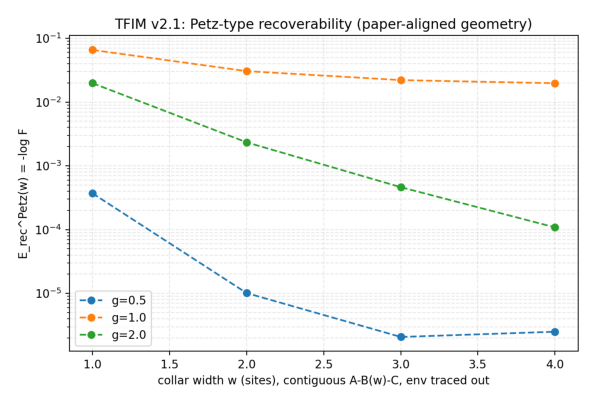
\includegraphics[width=0.55\textwidth]{fig1_tfim_control.png}
\caption{TFIM control (v1 figure, unchanged).}
\end{figure}

\section{First execution of the $\mathbb{Z}_2$ testbed (added in v2)}
\label{sec:z2}
v1 specified the gauge testbed but reported no gauge data. v2 executes a
minimal instance: a ladder of $P = 4$ plaquettes ($2 \times 5$ vertices,
13 links, qubits on links), $H(g) = -g\sum_\ell \sigma^x_\ell -
\tfrac{1}{g}\sum_p \prod_{\ell \in \partial p}\sigma^z_\ell$, Gauss law
enforced by a commuting penalty ($\lambda = 10$); ground states by sparse
Lanczos; EHS reduced states by partial trace over links.
\emph{Recoverability:} $A$ = leftmost rung (fixed), $B(w)$ = all links of
the first $w$ columns (admissible separation per the 2601.0043 v2
lesson), $C$ = the remainder ($|C|$ varies -- declared, as in the
original $d_{\rm eff}$ design); $\Erec(w)$, $w \in \{1,\dots,4\}$, by
exact pure-state low-rank evaluation. \emph{Wilson decay:} $\langle
W(1{\times}R)\rangle$, $R \in \{1,\dots,4\}$; on a height-one ladder,
area ($R$) and perimeter ($2R{+}2$) are degenerate, so the extracted
$\xi_W$ is the \emph{combined} Wilson decay length, declared as the
ladder proxy.

\begin{center}
\begin{tabular}{lllll}
\hline
$g$ & $\langle G_v\rangle_{\min}$ & $\xi_{\rm rec}$ ($n$ pre-floor) &
$\xi_W$ & comment \\
\hline
0.45 & 1.000000 & 0.221 (3) & 6.851 & \\
0.60 & 1.000000 & 0.203 (3) & 2.437 & \\
0.80 & 1.000000 & 0.274 (3) & 1.179 & \\
1.00 & 1.000000 & --- (2) & 0.798 & floor-limited \\
2.00 & 1.000000 & --- (1) & 0.383 & floor-limited (deep gap) \\
\hline
\end{tabular}
\end{center}

\begin{remark}[What the first dataset shows]
\label{rem:z2findings}
(i) The full pipeline -- Gauss sector, EHS reduced states, regularized
Petz, Wilson loops -- runs end to end with exact gauge invariance.
(ii) $\Erec(w)$ collapses to the numerical floor within one to two
columns at all sampled couplings: the ladder recoverability length is
very short ($\xi_{\rm rec} \approx 0.2$--$0.3$ lattice units) and nearly
coupling-independent (spread $\times 1.3$), while $\xi_W$ varies by
$\times 5.8$ over the same window (fittable couplings $g \in \{0.45, 0.6, 0.8\}$). \emph{At ladder level there is no
tracking between the two scales.} (iii) Because of the area/perimeter
degeneracy, $\xi_W$ on the ladder is not a pure confinement scale
(especially at $g < 1$), so this dataset is
\emph{inconclusive-but-cautionary} for the tracking conjecture, not a
falsification. (iv) The concrete lesson for the program: a resolving
test requires a genuine 2D lattice (e.g.\ $2 \times N$ or $3 \times N$
plaquette arrays), where Creutz ratios disentangle $\sigma$ from
perimeter terms and wider buffers postpone the numerical floor.
\end{remark}

\section{Verification suite (added in v2)}
\texttt{verification/2601-0044/verify\_2601\_0044.py} (sparse Lanczos;
chunked JSON cache; low-rank pure-state fidelities): Gauss-sector check,
$\Erec(w)$ profiles, Wilson decays, $\xi_{\rm rec}$/$\xi_W$ extraction
with the $n \ge 3$ identifiability policy, and the no-tracking summary of
Remark~\ref{rem:z2findings}. The v1 TFIM appendix script is kept
alongside.

\section{Discussion and outlook}
As in v1, updated: the open directions (fully algebraic sector-wise
implementation; comparison with string-tension proxies) now have a first
empirical anchor -- the executed ladder shows the protocol is sound and
cheap, and locates precisely where it must grow (2D geometry, floor
management, fixed-target variants per 2601.0043) before the tracking
conjecture can be meaningfully tested.

\section*{Note added in v2}
No v1 definition, conjecture or protocol step is changed. v2 adds:
(1) the first execution of the $\mathbb{Z}_2$ testbed
(Section~\ref{sec:z2}), with exact Gauss invariance and the
no-tracking-at-ladder-level finding, framed as inconclusive for the
tracking conjecture due to the declared area/perimeter degeneracy;
(2) the shared-control acknowledgment with 2601.0043 and the instability
flag on the $g = 0.5$ TFIM row (confirmed by regeneration in the
companion's v2); (3) series positioning (v1 cited only the forthcoming
AQFT companion); (4) the verification suite. \emph{Correction during
integration review:} an off-by-one in the suite's Hilbert-space size
(\texttt{NL} $= 3P{+}2 = 14$ instead of the correct $3P{+}1 = 13$ links
for the $P = 4$ ladder: $P{+}1$ rungs plus $P$ top and $P$ bottom rails)
left one qubit with no Hamiltonian term acting on it. Since the ground
state then factorizes as $\psi_{\rm ladder} \otimes \chi$ with $\chi$
pure, the spectator provably cancels in every reported observable
(Gauss, Wilson, and $\Erec$: the pure factor tensors through the Petz
map and the fidelity). The suite now uses $\texttt{NL} = 13$; all
regenerated numbers agree with the 14-qubit run up to floor-level
jitter, which shifted the fittable-coupling set from
$\{0.45, 0.6, 1.0\}$ to $\{0.45, 0.6, 0.8\}$ without changing any
finding.

\begin{thebibliography}{12}
\bibitem{ForthAQFT} L. Eriksson, \emph{Petz recoverability in AQFT via
conditional expectations}, preprint (2026).
\bibitem{Petz} D. Petz, Commun. Math. Phys. \textbf{105} (1986)
123--131.
\bibitem{FR} O. Fawzi and R. Renner, Commun. Math. Phys. \textbf{340}
(2015) 575--611.
\bibitem{Kogut} J. B. Kogut, Rev. Mod. Phys. \textbf{51} (1979) 659.
\bibitem{Donnelly} W. Donnelly, Phys. Rev. D \textbf{85} (2012) 085004;
Class. Quantum Grav. \textbf{31} (2014) 214003.
\bibitem{CHR} H. Casini, M. Huerta, and J. A. Rosabal, Phys. Rev. D
\textbf{89} (2014) 085012.
\bibitem{S0043} L. Eriksson, ai.viXra:2601.0043 (2026; v2 2026).
\bibitem{S0038} L. Eriksson, ai.viXra:2601.0038 (2026; v2 2026).
\bibitem{S0040} L. Eriksson, ai.viXra:2601.0040 (2026; v2 2026).
\bibitem{S0042} L. Eriksson, ai.viXra:2601.0042 (2026; v2 2026).
\bibitem{S0035} L. Eriksson, ai.viXra:2601.0035 (2026; v2 2026).
\end{thebibliography}
\end{document}
